\section{Results}\label{sec:results}
In this section, we provide the result of hedging BTC with BTC future using different copulae and risk measures.
The results is drawn using the data from 29/12/2017 to 27/05/2021 (15/12/2017 is the first trading day of the CME BTC future).
BTC price is obtained from Tiingo, a data provider who aggregate BTC prices of major exhanges in the market;
BTC future price is quoted by CME and retrieved as daily closing price from Bloomberg Terminal.
\medskip

Before estimating the optimal hedge ratio, we pre-process the data as follow.
First, we inner joint the daily BTC price and BTC future by date,
i.e. match the prices with date and discard the unmatched.
Then, we compute the log returns by $r_t = \log \frac{P_t}{P_{t-1}}$ where $P_t$ is the price of an asset at time time $t$.
We use this log return to estimate h and evaluate $h$’s performances. \medskip

After preprocessing the data, we search $h^*$ for each copula-risk-measure pairs as follow.
First, we compute the the marginal distributions by empirical CDF (ECDF) for each training dataset.
Each training dataset consists of 300 returns.
The ECDF is $\hat F(x) = \frac{1}{300}\sum_{n=1}^{300} r \cdot 1(r \leq x)$.
Then, we calibrate copulae with the marginal ECDF by the method of moments mentioned above.
Next, we draw samples from copula and, with the samples, numerically search for the $h^*$ which minimise the risk measure.
We draw one million samples from copula for each search.
The $h^*$ is then applied to the out-of-sample data.
The out-of-sample is the data of the consecutive 5 trading day to the training data (window size of $5$).
The $h^*$ is indexed with the first date of the out-of-sample data.
We then shift the data with $5$ trading days and repeat the procedure (step size of $5$). \medskip

\subsection{Profit and Loss}\label{subsec:empirical-results}

%Figure~\ref{fig:Gumbel} shows the result of the Gumbel-Variance.
%One can see that the fluctuation of the hedged log returns is smaller then that of the BTC and BTC future.
%The extreme negative returns (red dots) of BTC is well managed by the hedge. \medskip
%%One can see all the combinations of copula and risk reduction objective generate a large fluctuation of returns in
%%25/09/2019 and 26/09/2019.
%%This large fluctuation is due to dependence break.

Figure~\ref{fig:Gumbel} shows the time series of out-of-sample $r^h$ using the NIG factor copula with the
objective of reducing variance.
The red dots are the 30 most extreme negative returns in Bitcoin.
In the figure, we can see the downside risk of Bitcoin is well managed by the hedging procedure with NIG factor copula.
Most of the extreme losses of Bitcoin are greatly reduced by introducing the CME future in the hedged portfolio.
Two exceptions are found in 25/09/2019 and 26/09/2019, where the CME future failed to follow the large drop in Bitcoin.
%The reason of drop is unknown, but sudden drop in price is common in the cryptocurrency market.
One of the possible reason is that traders was performing rollover activities on 25-26/09/2019, which
27/09/2019 is the expiry day of the September future.
Another reason for the NIG factor copula fail of capturing the loss is dependence break.
The Kendall's tau in the training data is 0.2 higher than that of the testing data.
Other copulae suffer from the break as well. \medskip
%
\begin{figure}[th]
   \centering
   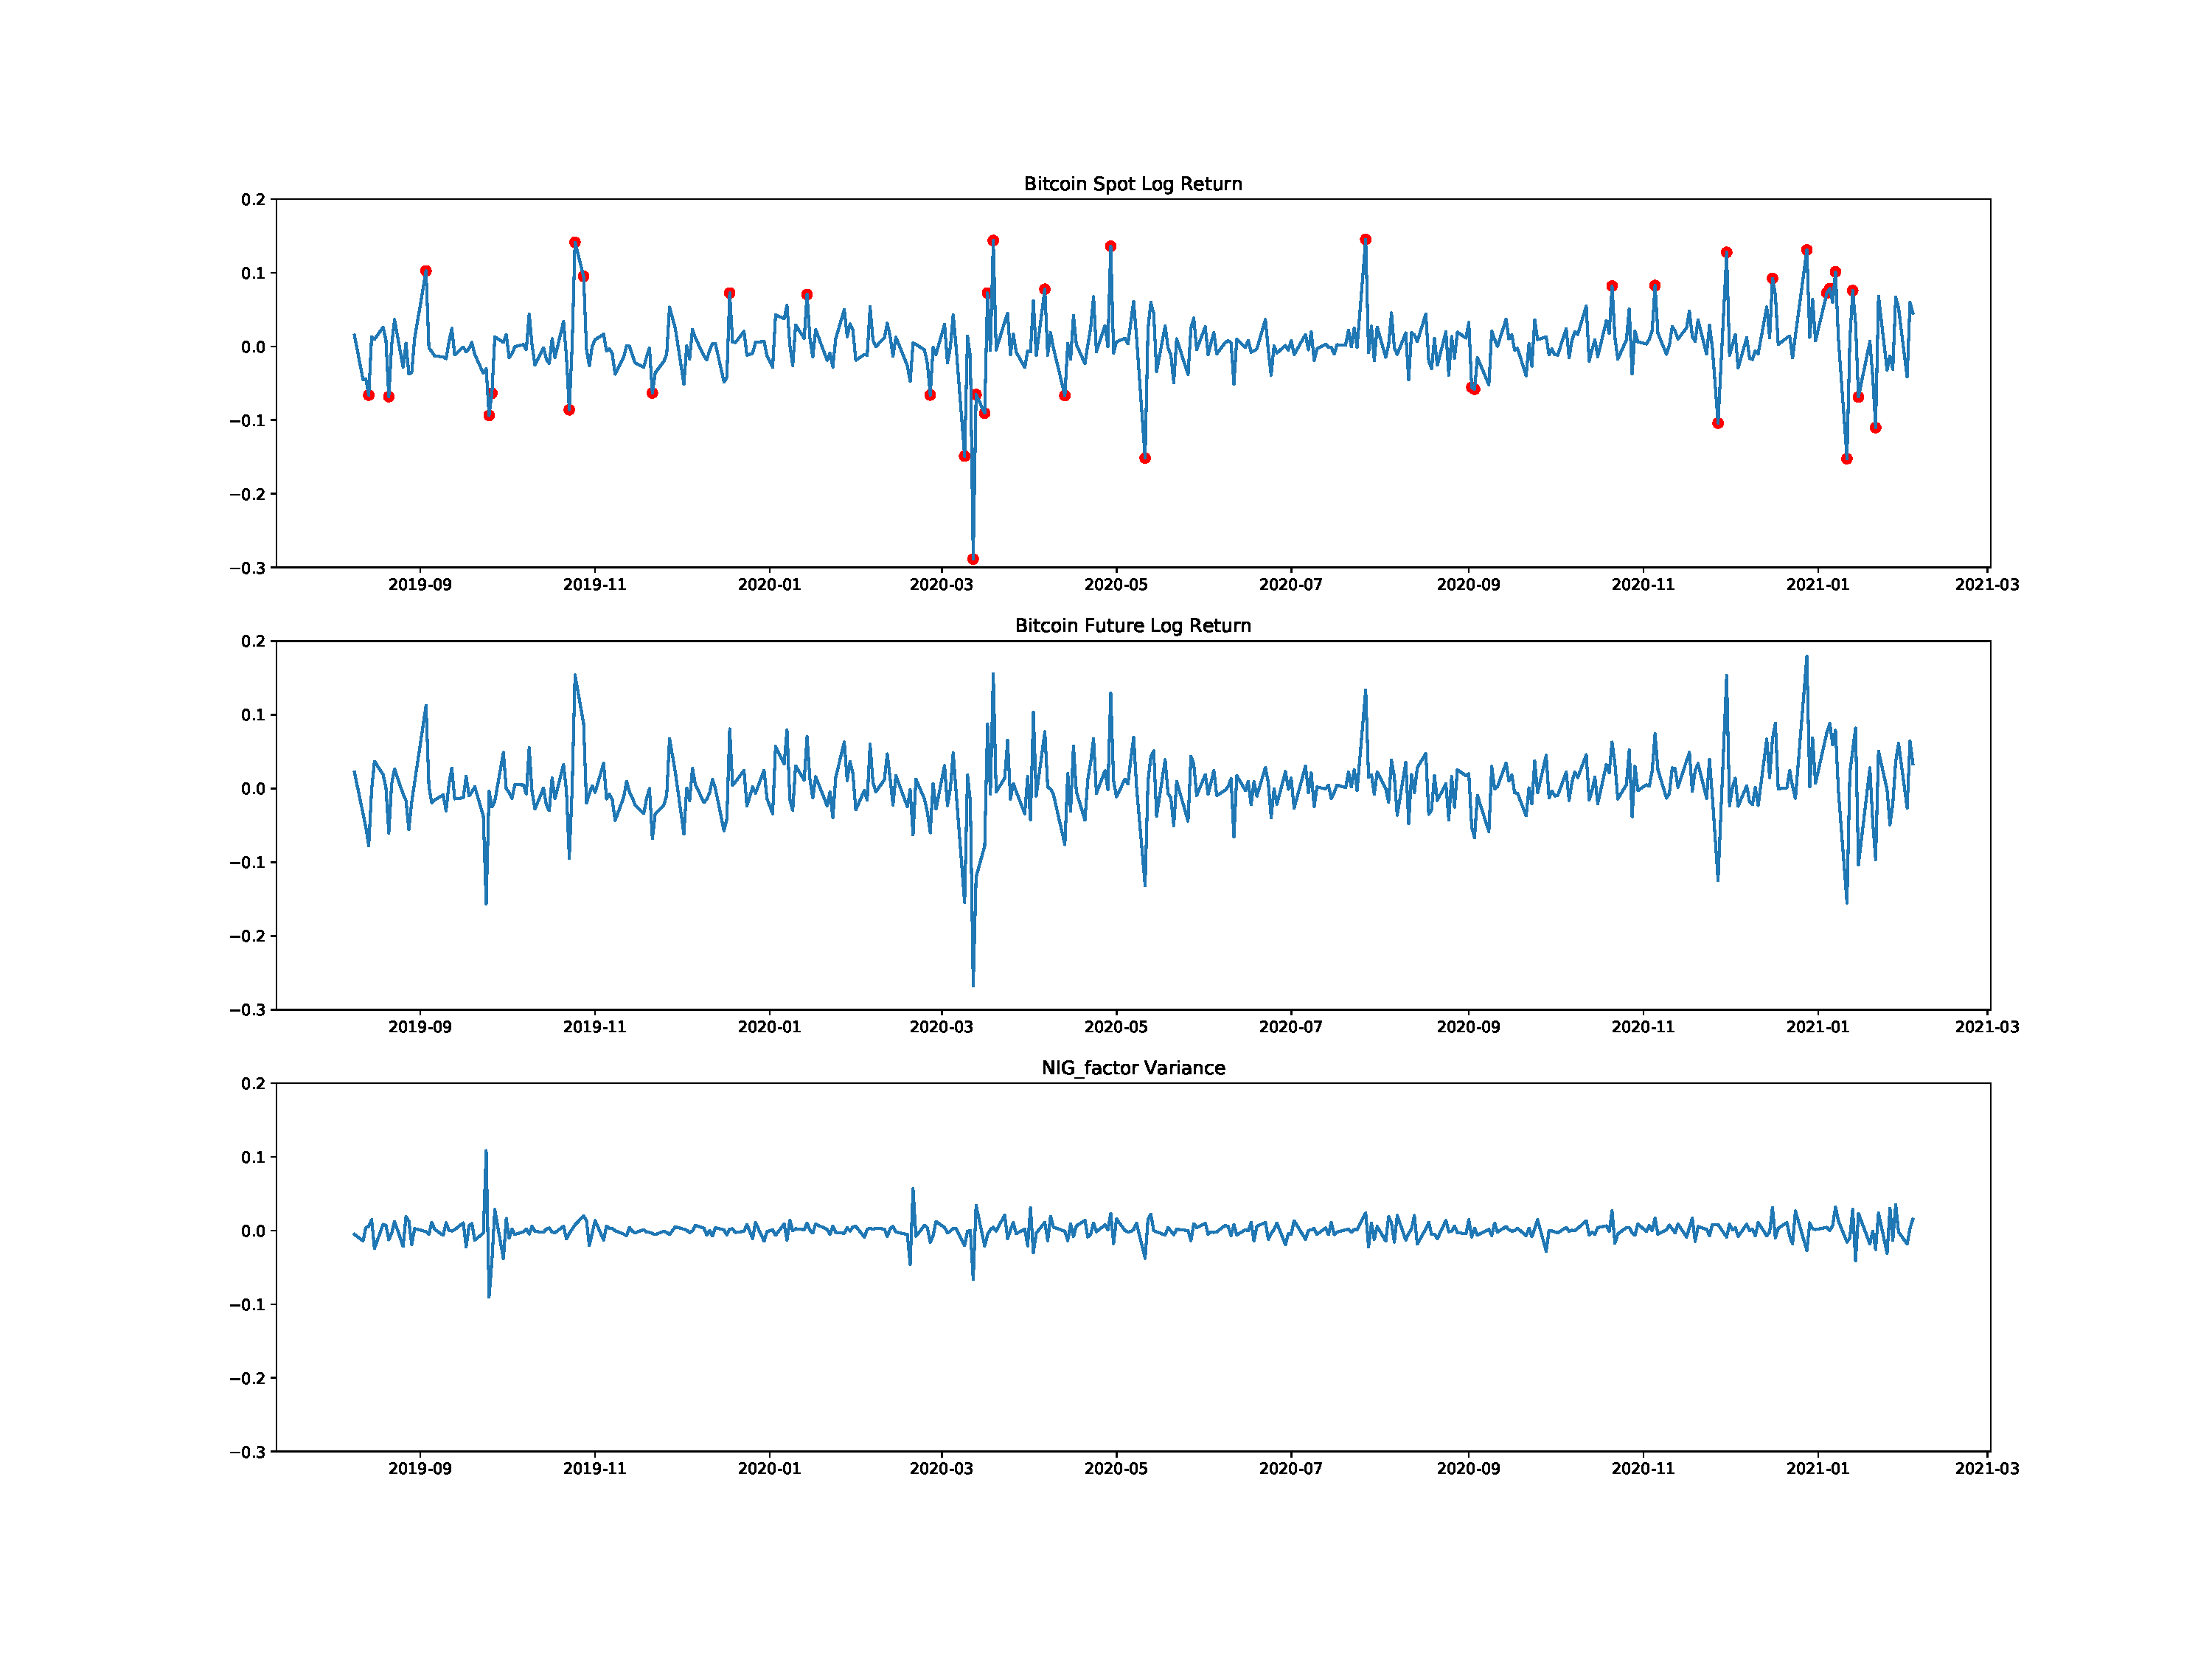
\includegraphics[width=\textwidth]{_pics/OOSreturns_compare.pdf}
   \caption{First Panel: Out of Sample Log-return of Bitcoin; Second Panel: Out of Sample Log-return of Future;
   Third Panel: Out of Sample Log-return of Hedged Portfolio by NIG factor copula with the aim of variance reduction.
   The red dots indicate the lowest 10\% return of Bitcoin, i.e. large negative moments of price.
%   Forth Panel: Out of Sample Log-return of Hedged Portfolio by $h=1$ (naive hedge).
%   Lower Panel: Out of Sample Hedged Portfolio log-returns.
%   The $h^*$ is obtained from Gumbel copula aiming at reducing variance.
%   The red dots indicate the 30 most extreme negative returns in Bitcoin.
   \href{http://www.quantlet.com/}{\includegraphics[width=20pt]{_pics/qletlogo_tr.png}}}
   \label{fig:Gumbel}
\end{figure}

Results of the other pairs are very similar, they are documented in
figure~\ref{fig:OOSRH} in the appendix.
The figure tabulates the time series of out-of-sample returns of hedged portfolio under various copulas and risk reduction objectives.\medskip

\subsection{Evaluation}\label{subsec:evaluation}
In addition to the PnL generated by different copula-risk-measure pairs,
we evaluate their performance by hedging effectiveness (HE), root mean squared error (RMSE), and downside semivariance (SV).
The purpose of evaluating performances of copula-risk-measure pairs beyond PnL is to assist the judgement of which pairs can estimate the optimal hedge ratio which
are suitable to hedge BTC with its future.
, in particular, HE measures the reduction of risk, the RMSE and SV relate investors' preference
(via utility function) while judging which random outcomes are better than the other.

%We illustrate the results in three directions, hedging effectiveness,
%ability of hedging extreme negative events in $r^S$, and the stability of $h^*$.

%\begin{itemize}
%   \item  Hedging Effectiveness
%   \begin{itemize}
%     \item Kick out Frank for its ineffectiveness; Alternative to a one-parameter symmetric Archimedean copula is Plackett;
%       \natp{\em [The issue with the Frank copula is that is has no
%         tails. A scatterplot looks like a strip, there is no
%         concentration in the tails. For CDO pricing (and this is what
%         I remember from my PhD studies) this poses problems as you
%         move from senior to junior tranches. Here, I suppose it just
%         does not capture the empirical behaviour of the data.
%         ]}
%     \item Differences among combinations of copula and risk reduction objective are small;
%     \item None of the combination can escape from the structural break point (dependence of training is stronger then that of testing). (The bump in 25-26th Sept 2019)
%     \item The best performing RRO of a particular risk measure in out-of-sample $r^h$ is not necessarily same, e.g.
%      VaR 95\% as RRO (with Gumbel copula) can generate the lowest out-of-sample ES 99\%.
%   \end{itemize}
%   \item Ability to hedge extreme events in $r^S$
%   \begin{itemize}
%     \item The extreme events in $r^S$ are well managed by the hedge.
%     The magnitudes of loss in $r^h$ is much smaller than that of $r^h$. (Visually seen from the time series of $r^h$)
%     \item None of the combination can escape from the structural break point (dependence of training is stronger then that of testing)
%   \end{itemize}
%   \item Stability of $h^\ast$
%   \begin{itemize}
%     \item Gumbel gives high $h$ all the time; the extreme events are "hedged" ex-ante.
%     \item ES 99\% and VaR 99\% as risk reduction objective are too sensitive to extremes in training data;
%     Large changes in $h$ are suggested in response to extremes training data, while the testing data are less extreme;
%     \item ERM can be seen as a smoothed risk measure focusing in the lower tail of $r^h$; Less sensitive to rare events; Suggested.
%   \end{itemize}
%\item \end{itemize}

\subsubsection{Hedging Effectiveness}\label{subsubsec:hedging-effectiveness}
The hedging effectiveness (HE) measures the reduction of portfolio risk.
This notion of evaluating of hedging performance was proposed by \citet{ederington1979hedging} in the context of hedging the newly introduced
organized futures market.\medskip

HE is defined as
\begin{align}
  1- \frac{\rho(r^h)}{\rho(r^S)},
  \end{align}
where $\rho$ is a risk measure.

We measure the HE of copula-risk-measure pairs according to the risk measure, for example we measure the
HE of Gaussian-ES99\% pair by
\begin{align}
  1- \frac{\text{ES}_{99\%}(r^h)}{\text{ES}_{99\%}(r^S)},
  \end{align}
where $r^h$ is out-of-sample return generated by Gaussian-ES99\%, and $r^S$ is the out-of-sample log return of BTC. \medskip

\begin{figure}[H]
   \centering
   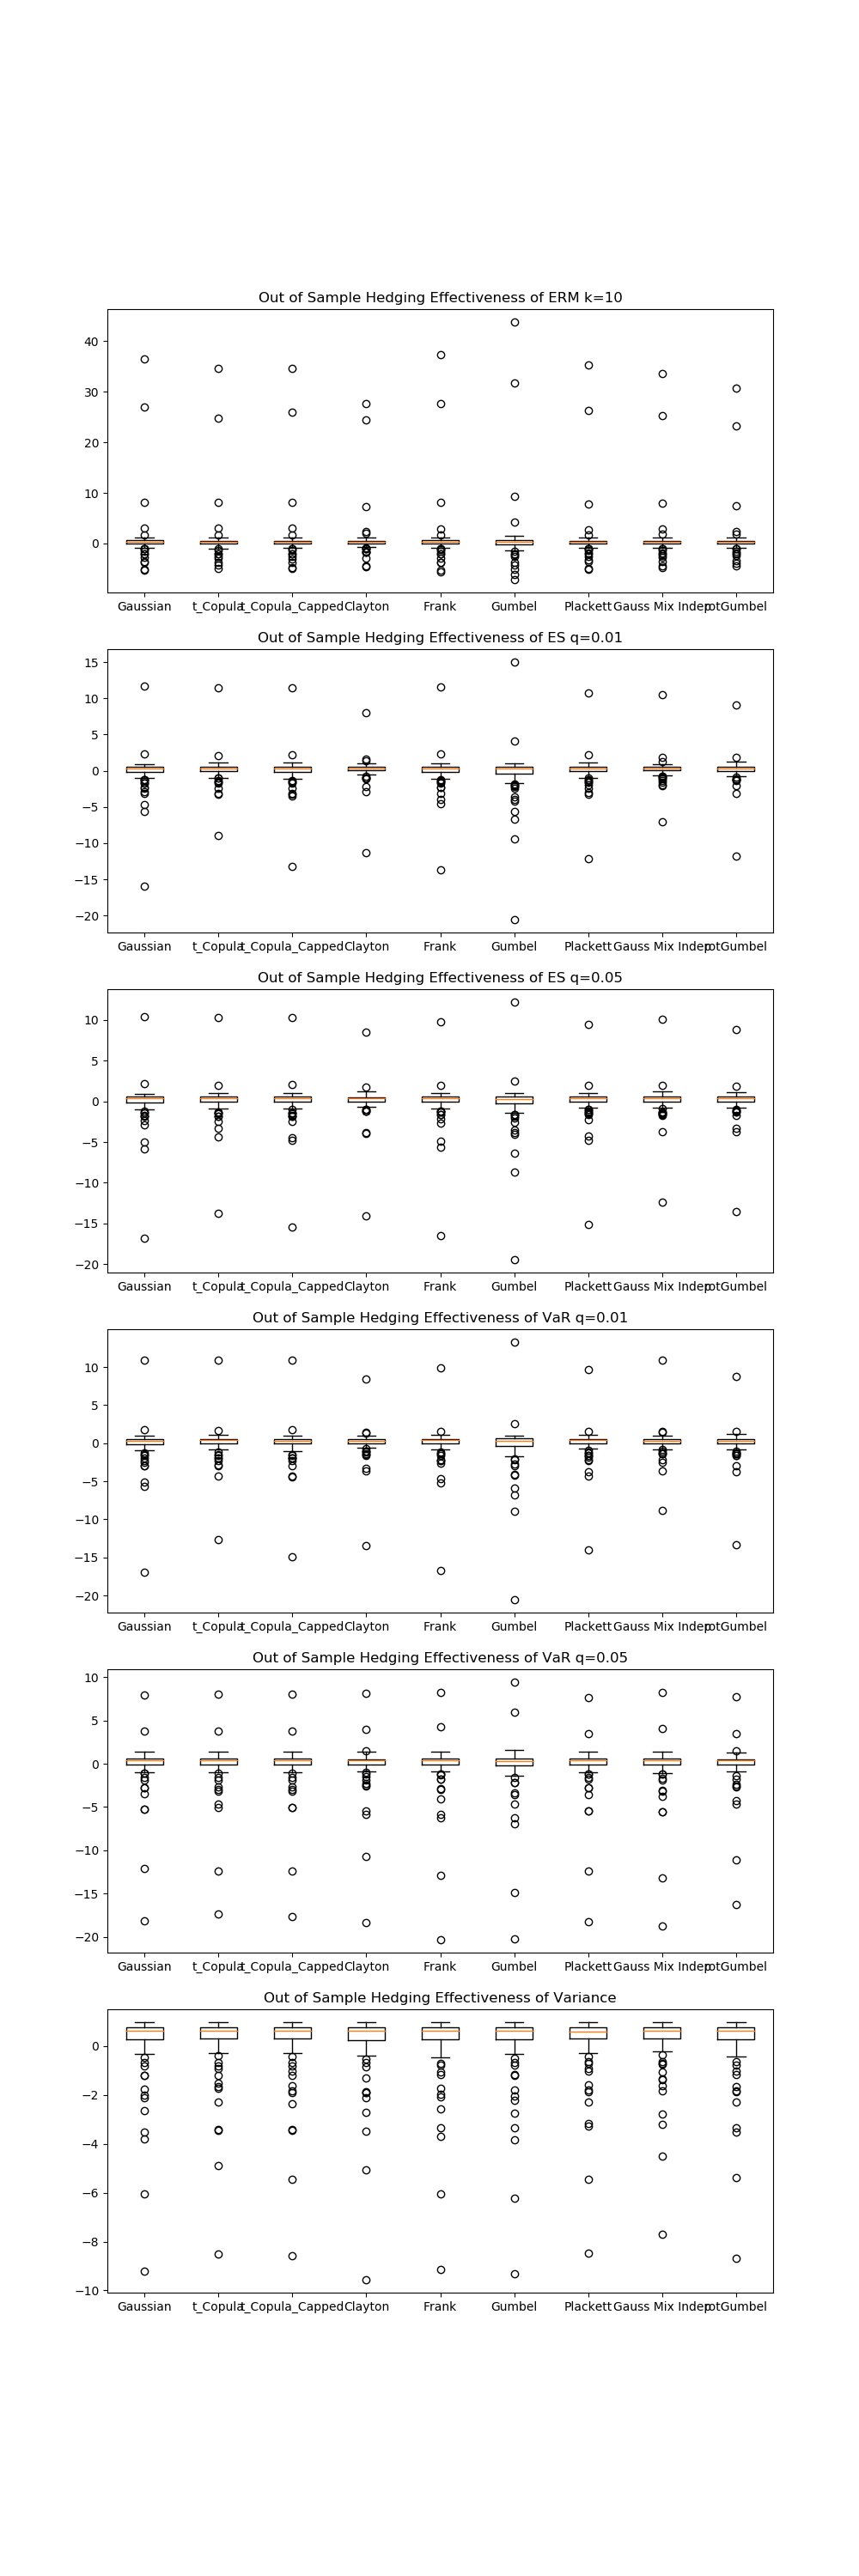
\includegraphics[height=24cm]{_pics/Out of Sample Hedging Effectiveness.png}
   \caption{Out of Sample Hedging Effectiveness Box-plot.
   The HEs are obtained from a set of out-of-sample data,
   each set consists 30 days log returns of Bitcoin and CME future.
   \href{http://www.quantlet.com/}{\includegraphics[width=20pt]{_pics/qletlogo_tr.png}}}
   \label{fig:OOSHE}
\end{figure}

The box-plots in figure \ref{fig:OOSHE} show the out-of-sample hedging effectiveness of different copulas under various risk
reduction objectives across testing datasets.
Observe that most of the copulae perform well.
The average HE of copulas and risk reduction objectives is higher than 60\% except for Frank-copula.
However, the HEs vary a lot in different testing data.
In some instances, the HE can be as low as 10\%.
This reflects the highly violate nature of cryptocurrencies:
the optimal hedge ratio in the training data deviates from that of testing data.
There is a large literature about structural break points and time changing dependence, to name a few
\citet{hafner2012dynamic}, \citet{patton2006modelling}, \citet{creal2008general},
\citet{engle2002dynamic}, \citet{giacomini2009inhomogeneous}, and also
\citet{manner2012survey}.\medskip

\subsubsection{Root Mean Squared Error and Semivariance}
Root mean squared error (RMSE) and semivariance (SV) are special cases of the Bernel Stone's generalized risk measure \citep{stone1973general}.
The purpose of applying a generalized risk measure is to measure the hedge performance of copula-risk-measure pairs in a common ground. \medskip

The Bernel Stone's generalized risk measure is
\begin{align*}
    \rho(F) = \int_{-\infty}^{\gamma(F)} \left|x-\eta(F)\right|^\alpha dF(x),
    \end{align*}
where $F$ is the distribution of the uncertain return, parameters $\alpha$ is chosen to represent preferences of investors,
$\eta(F)$ is a reference level of wealth from which deviations are measured, and $\gamma(F)$ is a range parameter that specifies the range of deviations to be included.\medskip

\citet{fishburn1977mean} justifies the usage of generalized risk measure (with his $\alpha$-$t$ model) by connecting the measure with Von Neumann-Morgenstern utility theorem, see also \citet{bawa1975optimal, bawa1978safety}
and \citet{morgenstern1953theory}.
We argue that evaluation of hedging performance of a crypto portfolio does not differ from this classical framework:
crypto investors maximise expected utility with given utility functions.
Vast body of recent literature remain in this classical framework, to name a few, \citet{sebastiao2020bitcoin, deng2020minimum, cui2020composite, oglend2020futures}. \medskip
See also \citet{chen2003futures} for a review of hedging performance evaluation.

%Hedging futures performance with denoising and noise-assisted strategies
%Minimum-variance hedging of Bitcoin inverse futures

For root mean squared error, we choose $\gamma(F)=\infty$ and $\eta(F)=0$, i.e. we consider a full range, from $-\infty$ to $\infty$, of deviations to our target
of zero PnL.
For semivariance (SV), we choose $\gamma(F)=0$ and $\eta(F)=\operatorname{\mathbf{E}}(r|r \leq 0)$.
The setting of semivariance represents our focus on the downside risk.
Sometimes, SV is called lower partial moment. \medskip

Therefore, for each pair of copula-risk-measure, we calculate
\begin{align*}
    \text{RMSE} = \operatorname{\mathsf{E}}\{(r-0)^2\}^{1/2},
    \end{align*}
and
\begin{align*}
    \text{SV} = \operatorname{\mathsf{E}}\left[\{r - \operatorname{\mathsf{E}}(r|r \leq 0)\}^2 | r \leq 0 \right].
\end{align*}

\begin{figure}%
    \centering
    \subfloat{{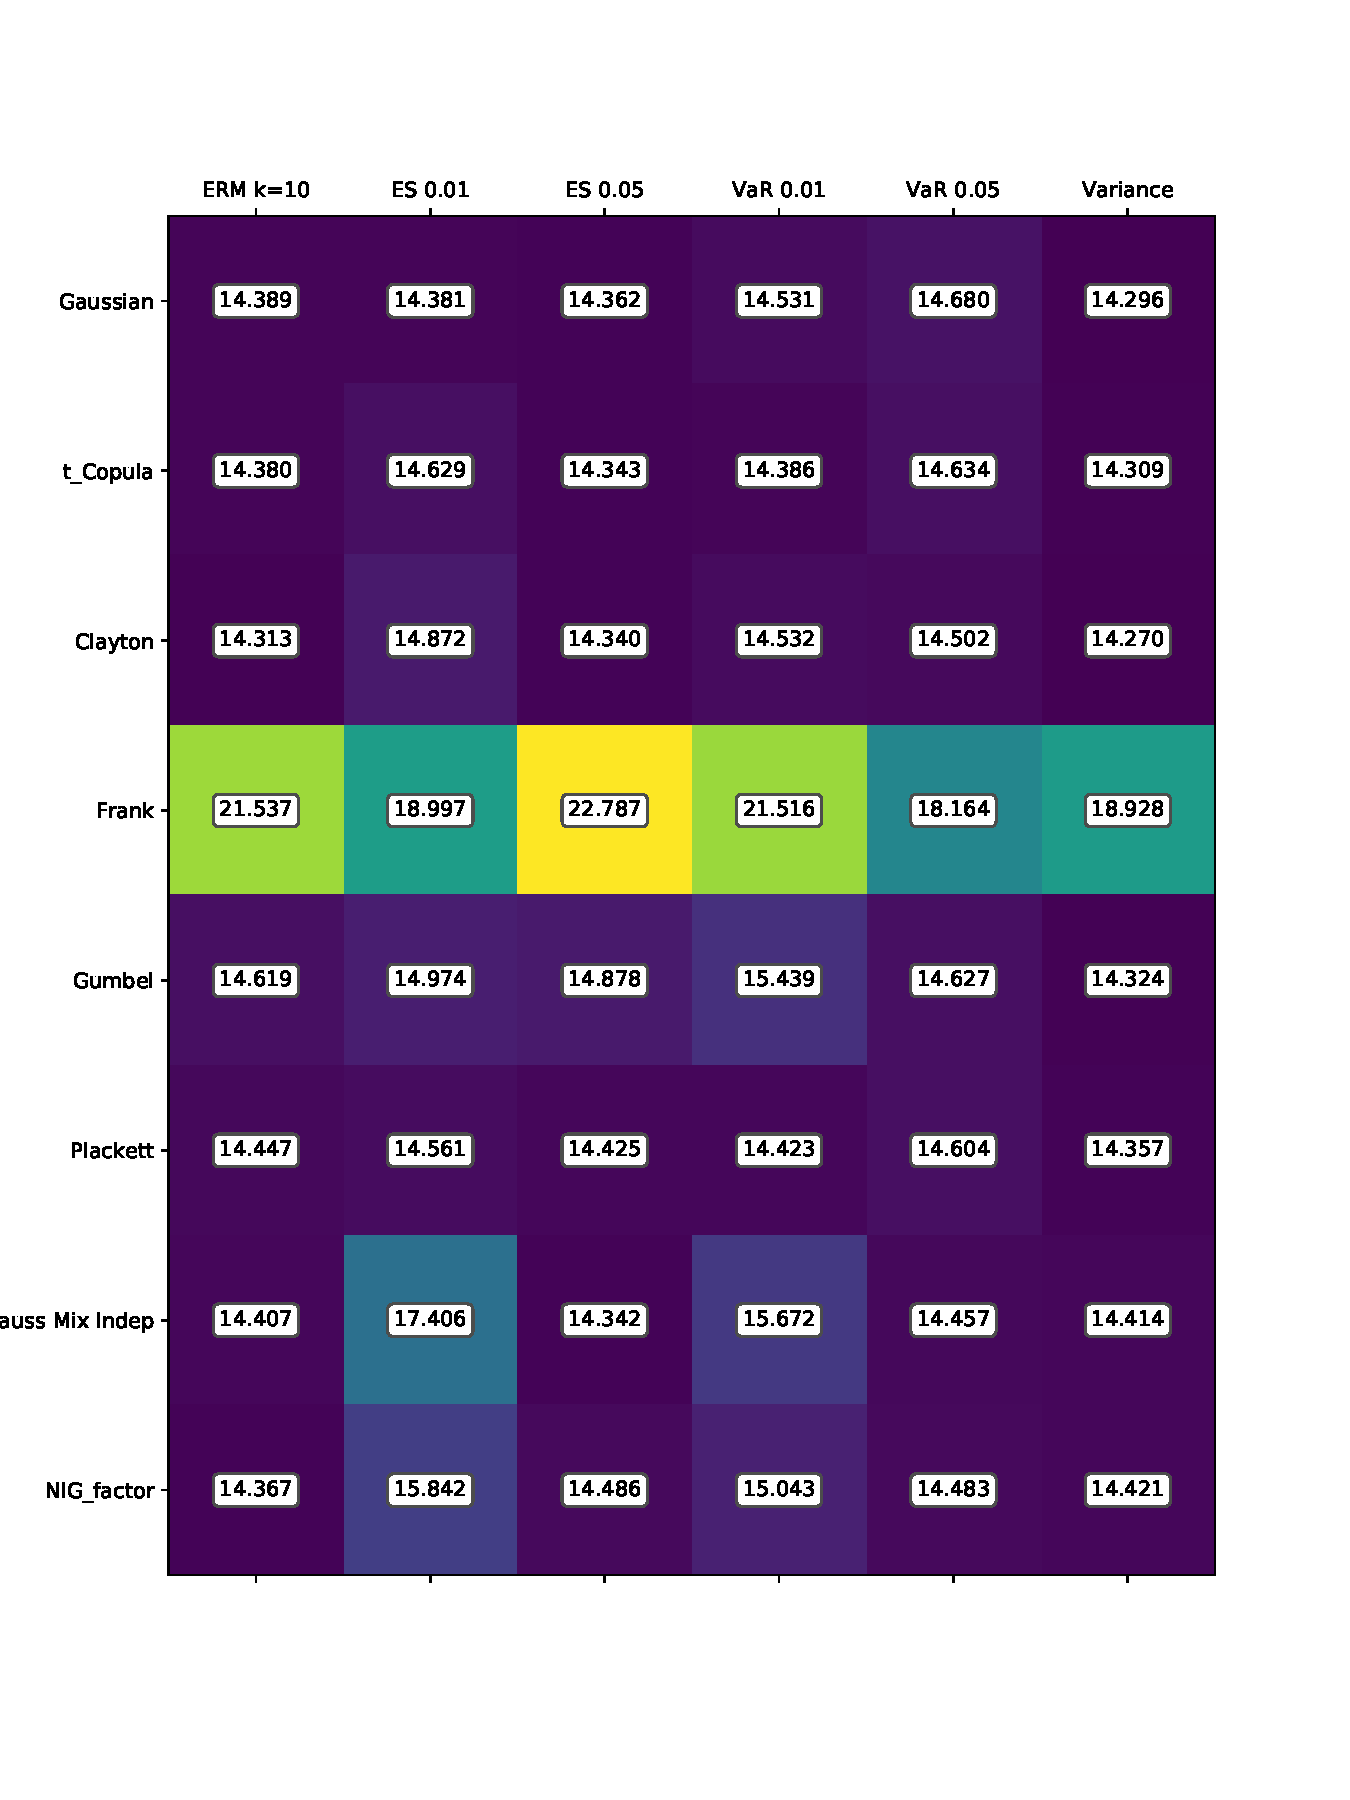
\includegraphics[width=.45\textwidth]{_pics/rmse_static.pdf} }}%
    \qquad
    \subfloat{{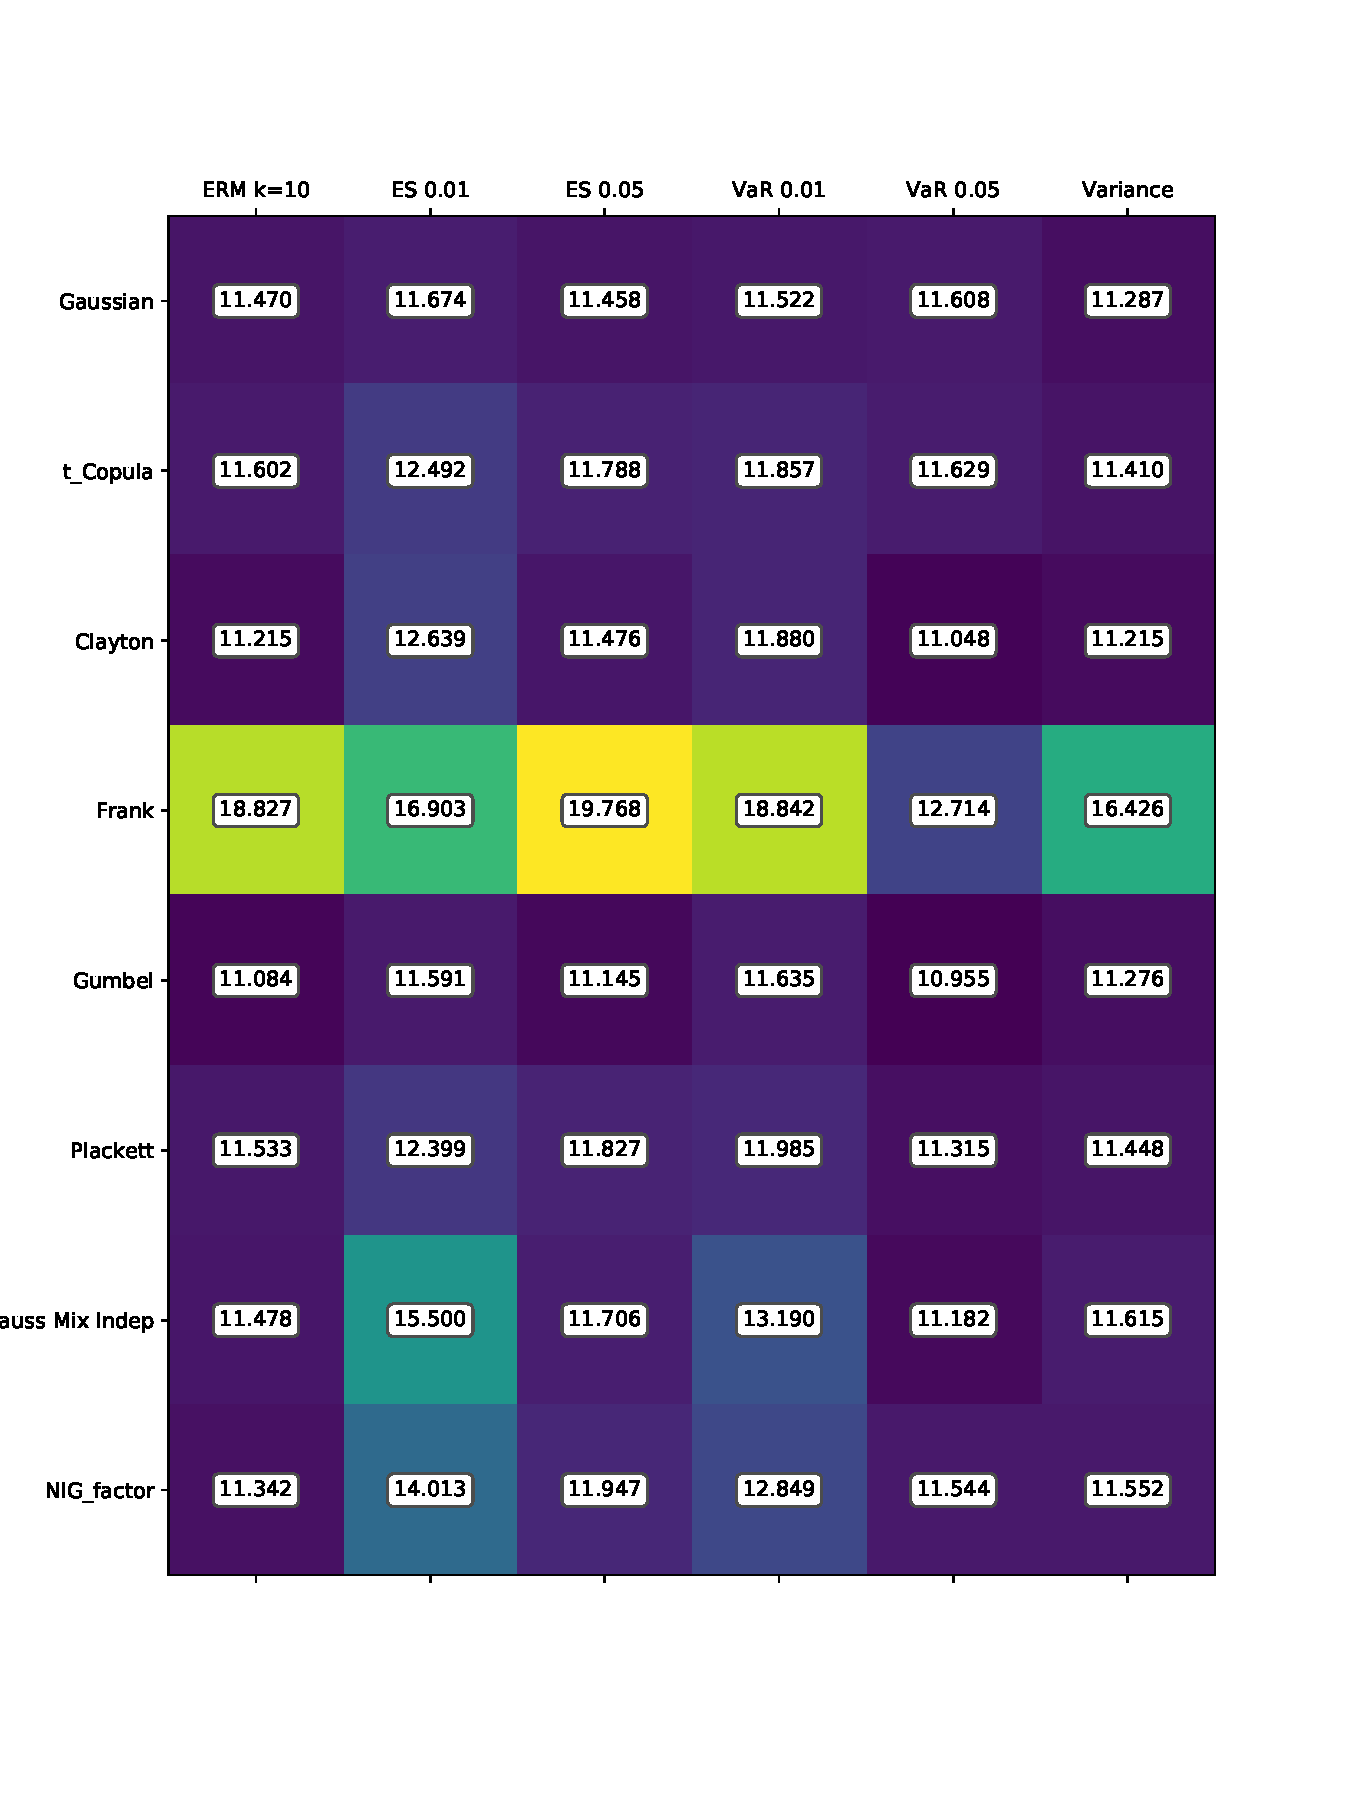
\includegraphics[width=.45\textwidth]{_pics/semivariance_static.pdf} }}%
    \caption{Left panel: RMSE$\cdot 1000$ of different copula-risk-measure pairs; Right panel: $\text{SV}^{0.5}\cdot 1000$ of
    different copula-risk-measure pairs. Frank copula is inferior to other copulae in terms of RMSE and SV.
    ES99\% and VaR99\% have slightly higher RMSE and SV.
%   Forth Panel: Out of Sample Log-return of Hedged Portfolio by $h=1$ (naive hedge).
%   Lower Panel: Out of Sample Hedged Portfolio log-returns.
%   The $h^*$ is obtained from Gumbel copula aiming at reducing variance.
%   The red dots indicate the 30 most extreme negative returns in Bitcoin.
   \href{http://www.quantlet.com/}{\includegraphics[width=20pt]{_pics/qletlogo_tr.png}}}%
    \label{fig:rmse_sv}%
\end{figure}

The result is shown in figure~\ref{fig:rmse_sv}.
The RMSE of the copula-risk-measure pairs is ranging from 0.014 to 0.023.
The smallest RMSE is generated by the pair Clayton-Variance, while a number of other pairs generate very similar results.
In particular, RMSEs of variance are relatively low while comparing with other risk measures across different copulae.
This is a natural result.
The Frank copula's RMSEs are high no matter the risk measures.
This suggests Frank should not be used to model the dependency structure of BTC and BTC future.\medskip

%RMSEs of VaR 99\% and ES 99\% across different copulae are also inferior to that of other risk measures.
%We will discuss this result in the robustness part. \medskip

The SV of the copula-risk-measure pairs is ranging from 0.011 to 0.020.
The best performing pair in terms of SV is Gumbel-VaR95\%.
Gumbel copula also has the lowest or second lowest SV while comparing with other copulae across different risk measures.
It is not surprising that Gumbel copula is superior than the other copula:
the dependency of positive jumps in BTC and BTC future is captured by Gumbel copula, while in our dataset,
positive jumps in BTC is frequent.
Furthermore, VaR95\% has the lowest or second lowest SV while comparing with other risk measure across different copulae.
Similar to the result in RMSE, various the copula-risk-measure pairs' SV performance are similar, except for Frank copula, VaR99\%, and ES99\%.

%\begin{figure}[t]
%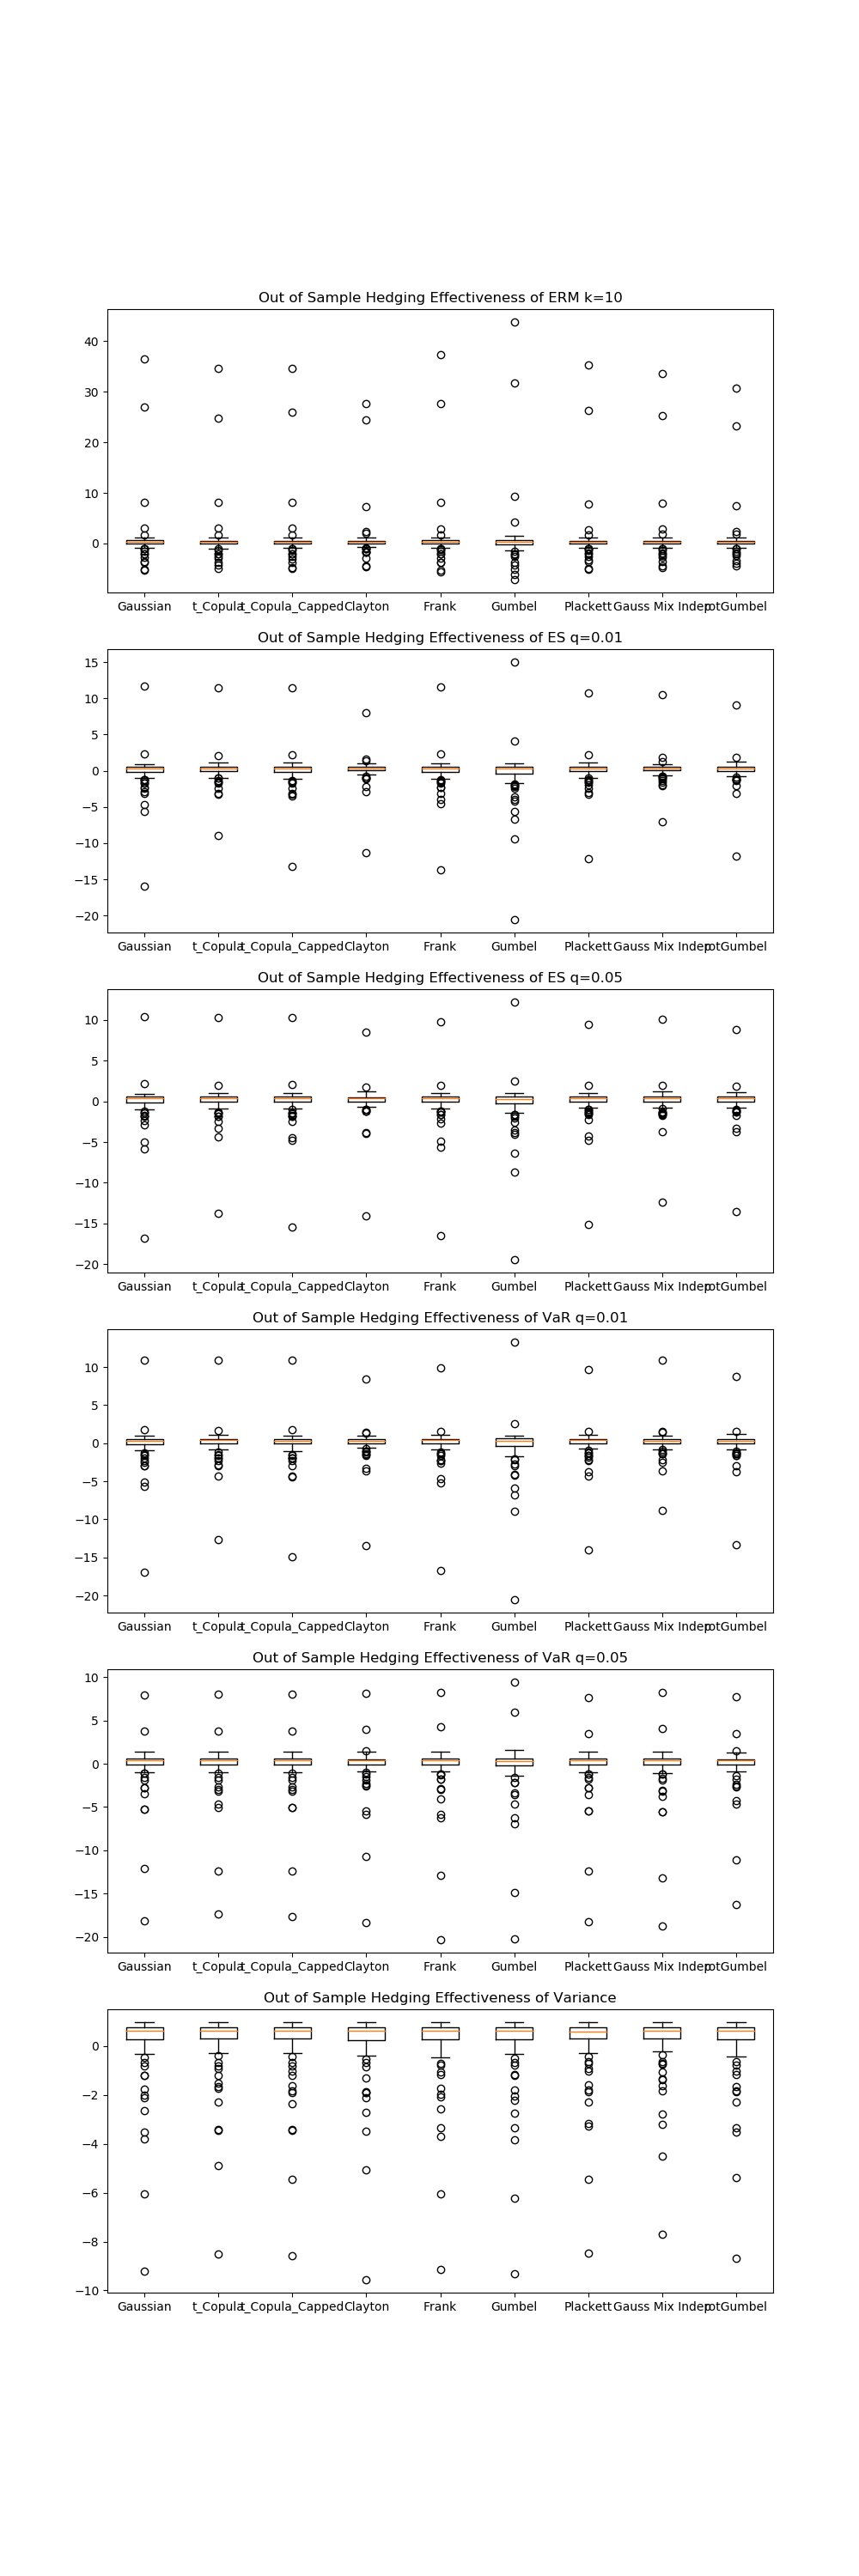
\includegraphics[width=\textwidth, height=\textheight]{_pics/Out of Sample Hedging Effectiveness.png}
%  \caption{}
%\label{out of Sample Hedging Effectieness}
%\end{figure}

%\subsubsection{Semivariance}
%Semivariance is a measurement of data to estimate the potential downside risk of an investment portfolio.
%It is the dispersion of all observations that is smaller than the mean or a certain threshold.
%Semivariance is discussed by many, to name a few,
%Markowitz (1959), Mao (1970a, 1970b),
%Mao (1970a), Hogan and Warren (1972, 1974).
%provide the theoretical justifications for semivariance.
%\subsection{Stability of $h^*$}

\section{Conclusion and Discussion}
In this paper, we model the dependency between Bitcoin (BTC) and its future via various copulae and search for
the optimal hedge ratios $h^*$ minimising different risk measures.
We conclude that various copulae, except the Frank copula, are appropriate to model the dependency structure between Bitcoin and its future when we want to minimise risk.
In addition, one should avoid using Value-at-Risk 99\% or Expected Shortfall 99\% as loss function while searching for the optimal $h^*$.
Other risk measures are ready to be deployed according one's objective.
The hedging effectiveness (HE) of various copula-risk-measure pairs are close to 65\%, i.e.
the risk of a portfolio of Bitcoin, measured by a particular risk measure, is reduced
by 65\% by including an optimal amount $h^*$ of Bitcoin future.
Again, the Frank copula is inferior to other copulae in terms of HE.
We also compare the root mean squared error (RMSE) and semivariance (SV).
Unsurprisingly, we can rule out the Frank copula, Value-at-Risk 99\% and Expected Shortfall 99\%
for hedging Bitcoin and its future.

\subsection{About Frank Copula}\label{subsec:Frank}
Frank-copula, in general, is not a good choice to model financial data.
We can see from figure~\ref{fig:Frank} that the Frank copula is not fitting the Bitcoin and its future visually, no matter
which optimization procedure is being deployed.
The samples of Frank diffuse like a strip with parallel edge when the parameter $\theta$ decrease (samples are being less dependent).
This makes Frank copula not a a good fit to the data.

\begin{figure}[th]
   \centering
   \includegraphics[width=\textwidth]{_pics/Frank.pdf}
   \caption{Comparison of Frank Copula Samples and Pseudo Observations of Bitcoin and CME Future Returns.
   \href{http://www.quantlet.com/}{\includegraphics[width=20pt]{_pics/qletlogo_tr.png}}}
   \label{fig:Frank}
\end{figure} \medskip

Aside from the Frank-copula, the HEs of various combination of copula and risk reduction objective are very similar.
This is an expected result as the portfolio consists only two assets.

\subsection{Robustness}\label{subsec:robustness}
The study of robustness concerns the stability of statistical estimation with respect to violation in assumptions.
In our context, the robustness is with respect to outliers (or jumps).
It is natural to do we want the optimal hedge ratio react to extreme market changes?
In practice, outliers of returns can come from anywhere, for example, a tweet from Elon Musk, a sudden large order from
institutional investor, or an incident of system failure in cryptocurrency exchanges.
Rapid and drastic changes in portfolio weight causes problem of slippage and transaction cost.
Investors should be aware of the cost brought by the sensitivity of the optimal hedge ratio procedure.
\medskip

The discussion of sensitivity or robustness dates back to \citet{huber1981robust}'s work on robust statistics.
\citet{hampel2011robust} suggest an infinitesimal approach to investigate sensitivity of statistical procedures.
There are three central concepts in this approach, qualitative robustness, influence function, and break-down point.
They are loosely related to the concept of continuity, first derivative of functional, and the distance of a functional to its nearest pole (singularity).
While the first concept is a qualitative feature of a functional, the second the third concepts are practical tools to measure sensitivity quantitatively.
We deploy a finite sample version of the second and third concepts.
Details of robustness of risk measures can be found in \citet{cont2010robustness}. \medskip

%\francis{\em [FL: Need to rewrite the following to show the IF of hedge performance instead of h. But Please have a look of the methodology first.]}
%With a probability space $(\Omega, \F, \p)$,
%we denote $M: \Omega \mapsto \mathscr{C}, M \in \{\text{MLE}, \text{MM}, \text{Empirical}\}$ be estimators of interest for distribution of returns,
%$$\mathscr{C} = \{\text{Gaussian-Copula}, ..., \text{Plackett-Copula}, \text{Empirical-Copula}\} \in \p$$ be a set of bivariate distributions of interest,
%$\rho_{h}: \mathscr{C} \mapsto \mathbb{R}$ be a risk measure on the hedged portfolio given $h$,
%and finally, $$\hat h_\rho = \argmin_h \rho_{h} \circ M$$ be a functional to obtain the optimal hedge ratio (OHR) depending on risk measure
%$\rho$. \medskip

The influence function of $\hat h_\rho$ with finite sample size $n$ is
\begin{align}
    \text{IF}(\bm{z}; \hat h_\rho) = \frac{\hat h_\rho(\bm{X}_1,...,\bm{X}_n, \bm{z})-
    \hat h_\rho(\bm{X}_1,...,\bm{X}_n)}{\frac{1}{n+1}}.
    \end{align}

%\francis{\em [The inclusion of $\bm{z}$ has nothing to do with the probability in a probability space, i.e. it is possible to include points with density zero.]}

The equation describes the effect of a single contamination at point $\bm{z}$ on the estimate of OHR,
standardised by the mass of the contamination. \medskip

Figure~\ref{fig:IFs} shows the influence function of $\hat h_\rho$ of using $t$ copula estimated by MLE with 300 data points of
Bitcoin and CME future returns from 14/12/2018 to 25/02/2020.
Contamination are in a set $\{-0.3,-0.27,..., 0.3\} \times \{-0.3,-0.27,..., 0.3\}$, in total $900$ pairs of contamination.
The product is Cartesian product of two sets.\medskip

We can see from the plots that Expected Shortfall with $\alpha = 99\%$ is very sensitive the negative return in spot (lower right plot).
The $h^*$ obtained this way increases with a single contamination of negative jump in spot price.
VaR at $99\%$ is also sensitive to negative jump in spot price but with a lower level (lower left plot).
This is a natural result that reflects investor's strong preference on risk avoidance: investor increases her future's short position
to compensate a large drop in spot price she saw in her data.
The result of ES being more sensitive to VaR as risk measure agrees with the conclusion of \citet{cont2010robustness}. \medskip

Other risk measures are relatively less sensitive.
Interestingly, although ERM places heavy weights to negative returns,
its IF is similar to that of variance, where variance does not exhibit risk preference.
%\francis{[FL:This might due to the smooth $\phi(p)$ over the spectrum $[0,1]$ of ERM. The $\phi(p)$ of VaR is a Dirac function at a single point $\alpha$, that of ES
%has a sharp cut off at $1-\alpha$, a tiny change in rank of $r^h$ (caused by a contamination $\bm{z}$) causes VaR and ES to shift their weights.]}

\begin{figure}[h!t]
      \centering
   \begin{tabular}[width=20cm, height=20cm]{ccc}
             \centering
   \includegraphics[height=5cm]{_pics/IF_plots/Variance_t_copula_MLE.pdf} &
   \includegraphics[height=5cm]{_pics/IF_plots/ERM10_t_copula_MLE.pdf}&
   \includegraphics[height=5cm]{_pics/IF_plots/VaR5_t_copula_MLE.pdf} \\
   \includegraphics[height=5cm]{_pics/IF_plots/VaR1_t_copula_MLE.pdf} &
   \includegraphics[height=5cm]{_pics/IF_plots/ES5_t_copula_MLE.pdf} &
   \includegraphics[height=5cm]{_pics/IF_plots/ES1_t_copula_MLE.pdf}
   \end{tabular}
   \caption{Influence functions (IF) of $h^*$ using $t$ copula copula estimated by MLE. From left to right, top to bottem, the plots are
   IF of using $\text{Var}$, $\text{ERM}_{10}$, $\text{VaR}_{0.95}$, $\text{VaR}_{0.99}$, $\text{ES}_{0.95}$, and $\text{ES}_{0.99}$ respectively.
   \href{http://www.quantlet.com/}{\includegraphics[width=20pt]{_pics/qletlogo_tr.png}}}
   \label{fig:IFs}
\end{figure}



%We measure the stability of $h^*$ by sum of absolute change
%\begin{align}
%    \sum_{t=1}^T|h_t - h_{t-1}|.
%    \end{align}
%
%Adjustment of portfolio weights induces price slippage (ref) and transaction cost.
%From figure \ref{SAD} we know the NIG factor copula with variance as risk reduction objective generates the smallest
%sum of absolute change in OHR.
%
%\begin{figure}[!th]
%   \centering
%   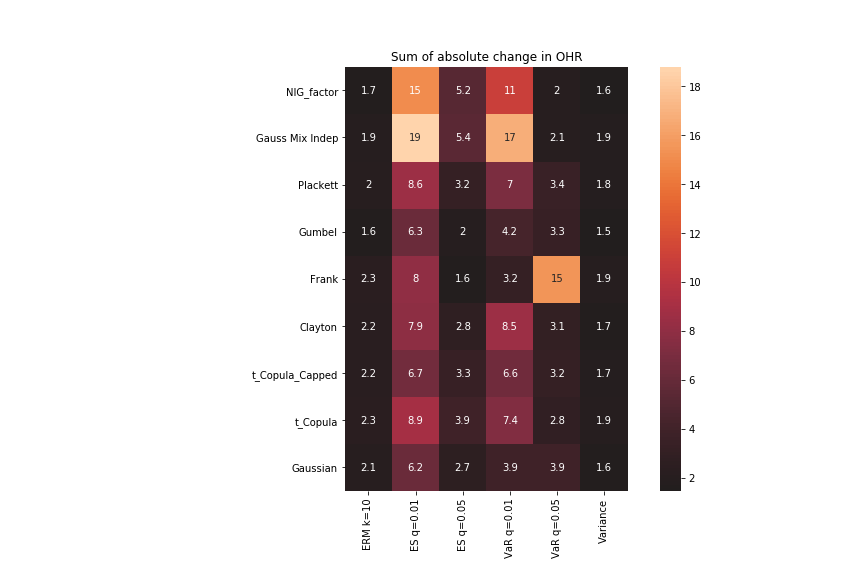
\includegraphics[width=\textwidth]{_pics/Sum of absolute change in OHR.png}
%   \caption{Sum of Absolute Change in OHR.
%   \href{http://www.quantlet.com/}{\includegraphics[width=20pt]{_pics/qletlogo_tr.png}}}
%   \label{fig:SAD}
%\end{figure}

%\input{table.tex}


